\documentclass[10pt,a4paper]{article}
\usepackage[UTF8,fontset=windows]{ctex}
\usepackage[margin=15mm]{geometry}
\usepackage{graphicx}
\usepackage{hyperref}
\hypersetup{hidelinks}
\setlength{\parindent}{0pt}
\setlength{\parskip}{4pt}
\begin{document}
\section*{图1　问题一：分时电价、供需与储能调度}
\begin{center}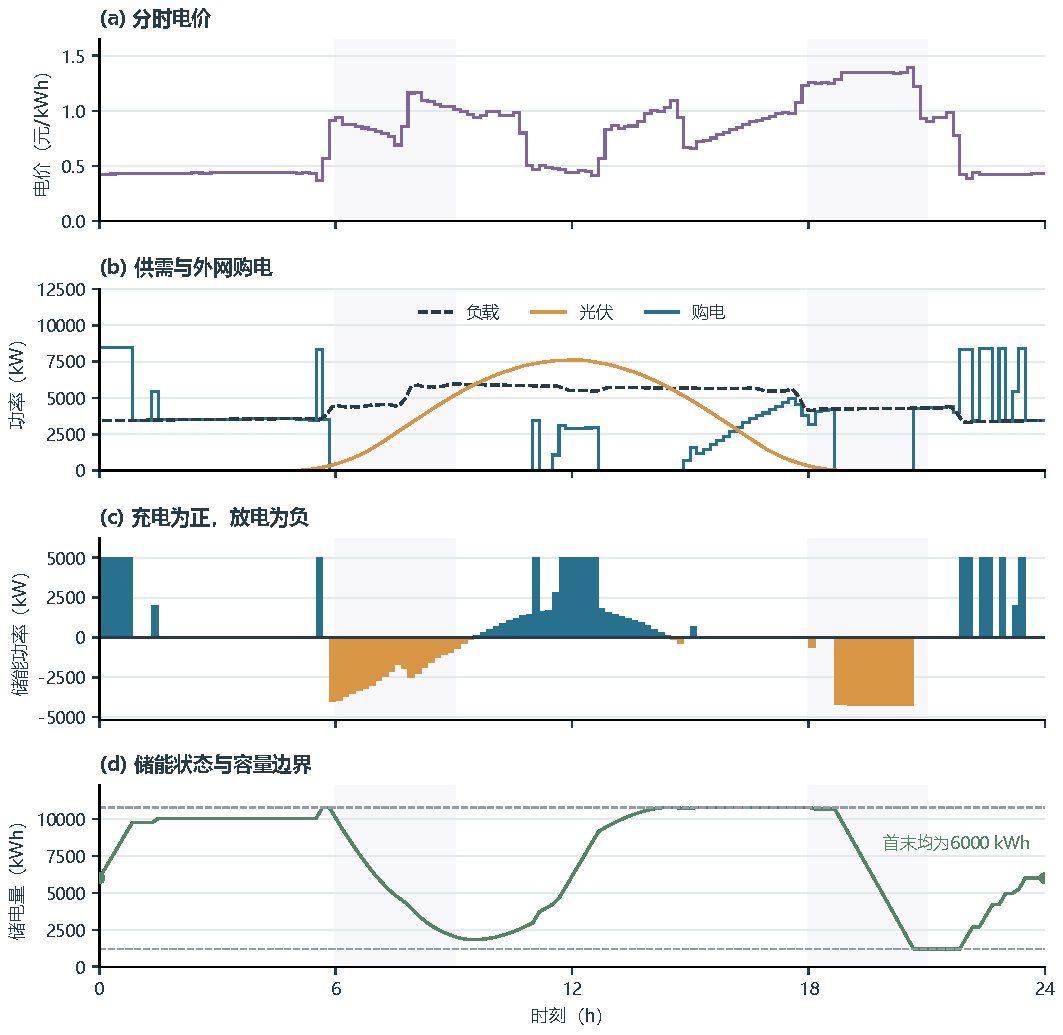
\includegraphics[width=\linewidth]{figures/01_q1_dispatch.pdf}\end{center}
{\small\textbf{图注：}典型日确定性调度结果。四个面板共享时间轴，依次展示电价、供需与购电功率、储能充放电功率及储电量；水平虚线为1200和10800 kWh的储电量边界，浅色背景仅辅助定位早晚时段。\par}
\medskip
{\small\textbf{正文描述：}在已知电价、负载和光伏的典型日中，优化购电费为35,126.95元。储能在部分低价时段及光伏富余时段充电，在高价时段放电；购电与充放电的联合安排改变了电量的时段分布。储电量始终位于规定区间内，且日初、日末均为6000 kWh，因此该收益并非通过消耗日初库存获得。\par}
\newpage
\section*{图2　问题一：购电转移与费用节省的账面分解}
\begin{center}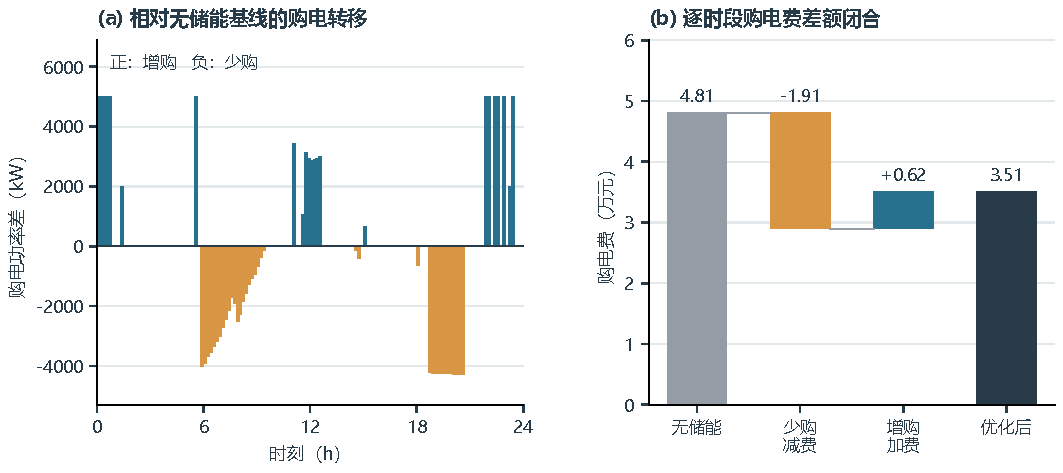
\includegraphics[width=\linewidth]{figures/02_q1_savings.pdf}\end{center}
{\small\textbf{图注：}储能调度相对无储能基线的购电差异与费用桥接。左图为优化购电功率减去无储能购电功率；右图按同一时段电价分别累计少购所减少的费用和增购所增加的费用。\par}
\medskip
{\small\textbf{正文描述：}无储能时的购电费为48,052.05元。储能使部分时段少购电，对应费用减少19,111.64元；同时在另一些时段增购电，对应费用增加6,186.54元。两者抵消后净节省12,925.10元，降幅为26.90\%。这一分解是逐时段购电费差额的恒等核算，不将同一节省进一步归因为独立的“光伏消纳效应”或“套利效应”。\par}
\newpage
\section*{图3　问题二：残差样本口径、成本权衡与启动期收益}
\begin{center}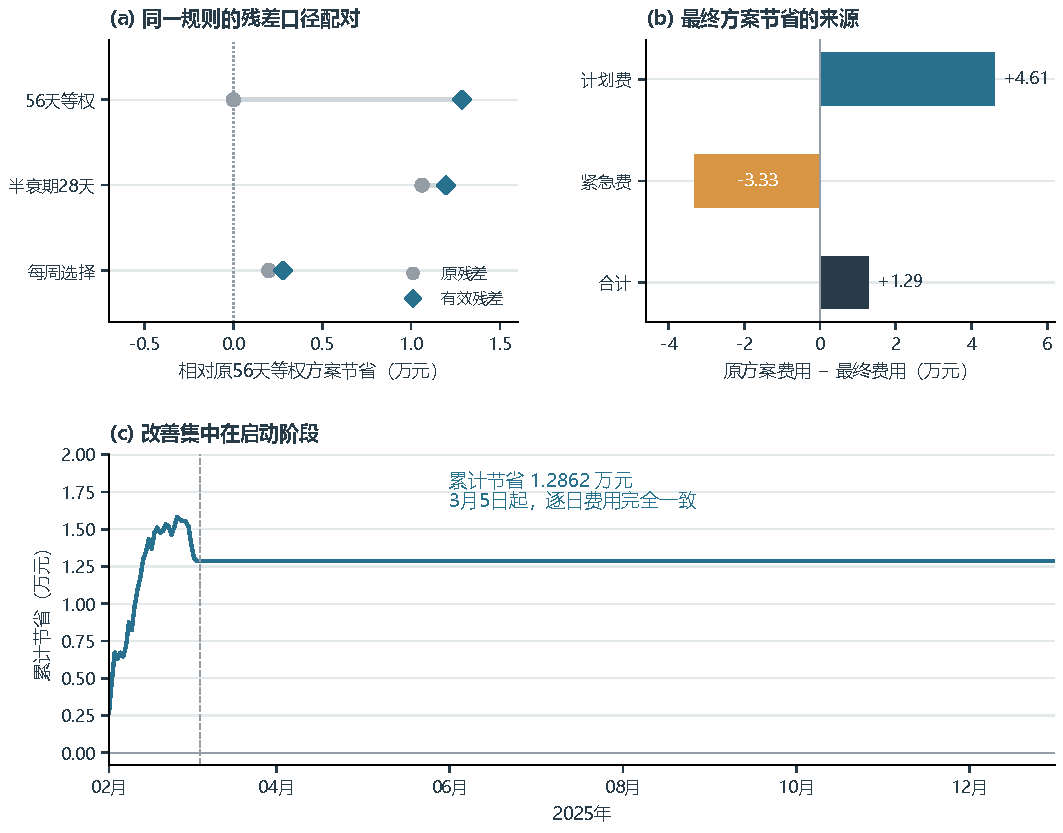
\includegraphics[width=\linewidth]{figures/03_q2_residuals.pdf}\end{center}
{\small\textbf{图注：}残差口径的配对比较及最终方案相对原方案的费用变化。(a)连线连接同一窗口规则在两种残差口径下的年度费用点，不是置信区间；(b)分解计划费与紧急费的节省；(c)展示全年累计节省。\par}
\medskip
{\small\textbf{正文描述：}在具有两种残差口径的三种窗口规则中，排除1月1—7日回退预测残差后，56天等权方案的回测费用最低，为14,389,135.08元。最终方案计划费减少46,129.24元，紧急费增加33,267.35元，净节省12,861.89元。累计收益于启动阶段形成，3月5日至12月31日逐日费用与原方案一致。因此，该改进应解释为残差样本口径调整在启动期的作用，不能据此声称全年持续适应能力提高，也不能据同年回测证明56天窗口对其他年份最优。\par}
\newpage
\section*{图4　问题三：预报融合与日内调整的逐级收益}
\begin{center}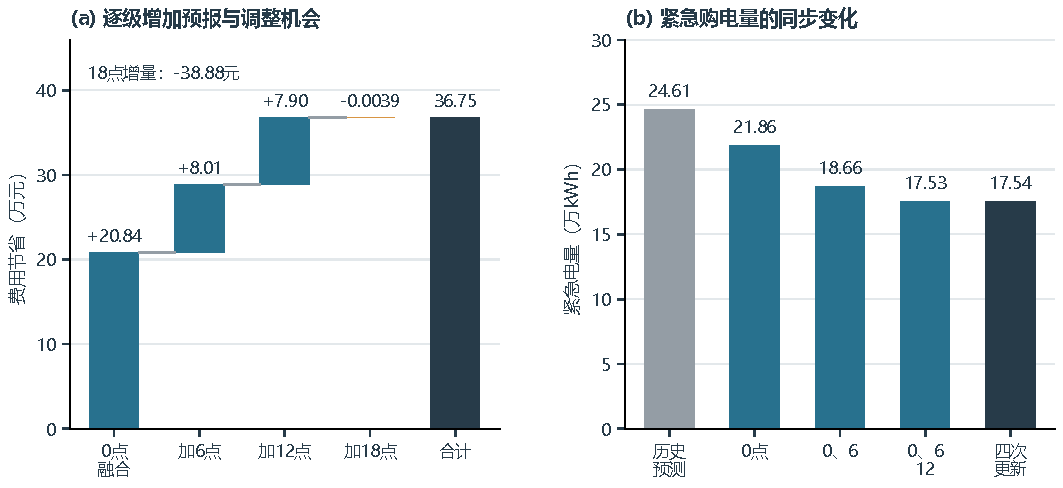
\includegraphics[width=\linewidth]{figures/04_q3_information_value.pdf}\end{center}
{\small\textbf{图注：}固定电价情形下的逐级费用节省与紧急购电量。费用节省以本问同口径历史预测对照为起点，依次引入0点融合预报和6、12、18点调整；右图按相同顺序比较紧急购电量。\par}
\medskip
{\small\textbf{正文描述：}四次更新主方案的总费用为14,022,396.98元，相对本问同口径历史预测对照节省367,495.52元。仅引入0点融合预报节省208,447.47元，随后增加6点和12点更新分别节省80,073.56元和79,013.36元；增加18点后费用变化为+38.88元，本年度未显示明确的额外经济收益。四次更新仍作为预设主方案保留。有限经验场景、重新聚类及滚动执行使真实回测费用不必随更新机会增加而严格下降。\par}
\newpage
\section*{图5　问题三：预报融合误差与权重变化}
\begin{center}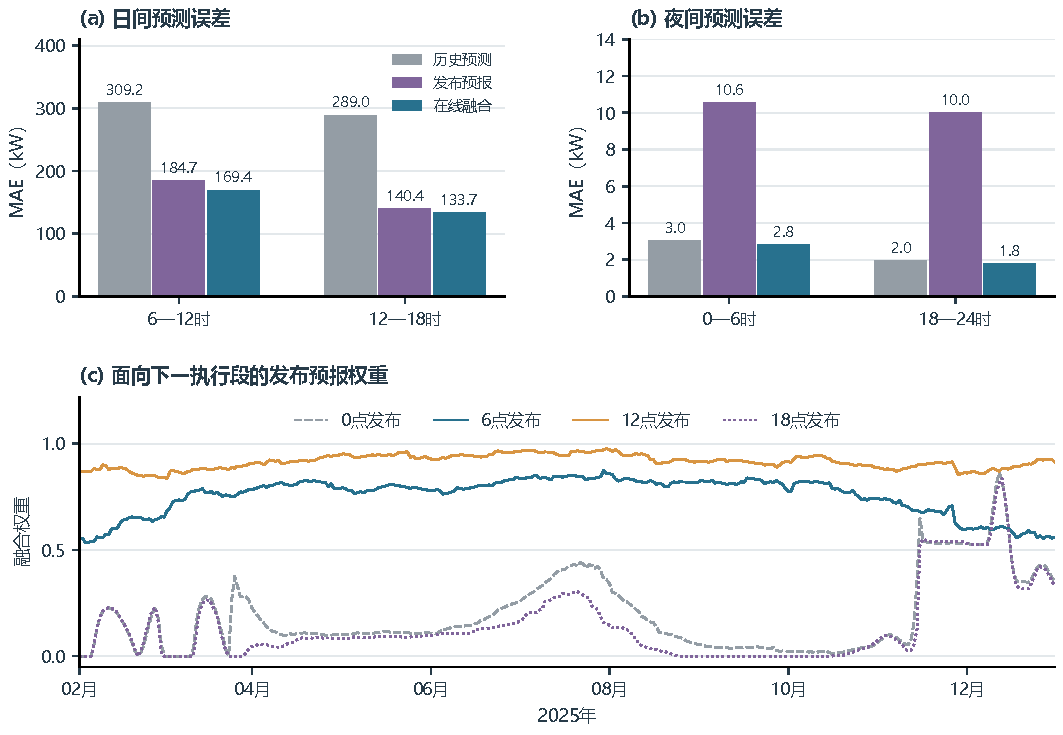
\includegraphics[width=\linewidth]{figures/05_q3_forecast_fusion.pdf}\end{center}
{\small\textbf{图注：}发布后六小时光伏预测误差及融合权重。(a)(b)分别比较日间和夜间的历史预测、发布预报及在线融合MAE，两面板纵轴尺度不同；(c)展示各发布时间对应的发布预报权重。\par}
\medskip
{\small\textbf{正文描述：}6—12时段的MAE由历史预测的309.24 kW降至融合预测的169.41 kW，12—18时段由288.99 kW降至133.68 kW。夜间绝对误差较小，单独绘制以保留其变化尺度。融合权重随历史已成熟样本更新，并包含原算法的偏差修正，因此融合输出不只是当期两条预报的固定加权平均。MAE改善本身不等同于等比例的费用下降，经济效果需结合更新频率对照判断。\par}
\newpage
\section*{图6　问题三：日内购电修正及储能衔接}
\begin{center}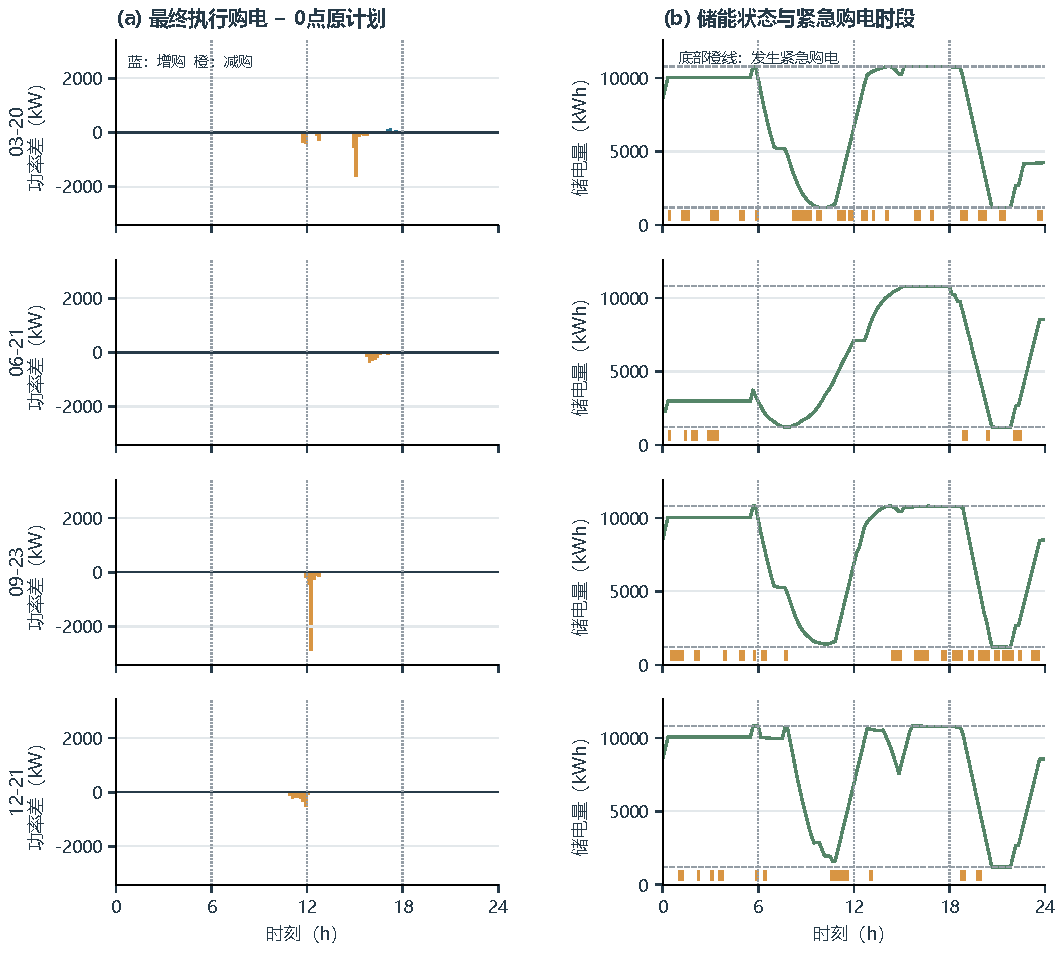
\includegraphics[width=\linewidth]{figures/06_q3_rolling_adjustment.pdf}\end{center}
{\small\textbf{图注：}四个指定日的日内计划修正与储能状态。左列为最终执行购电相对0点原计划的功率差，正值为增购、负值为减购；右列为储电量，底部橙色短线标记紧急购电大于数值容差的时段。竖虚线表示6、12、18点发布时刻。\par}
\medskip
{\small\textbf{正文描述：}日内更新后的购电修正相对原计划较小，直接叠加两条绝对购电曲线容易掩盖变化。以原计划为零基准后，可以清楚识别各执行区间内的增购和减购。储电量按跨日滚动过程衔接，指定日的首末电量不要求逐日相等。紧急购电标记说明计划与储能联合执行后仍可能存在实际供需缺口；该标记只表示发生时间，不表示缺口大小，也不能据其与储能状态的相邻关系断言单一原因。\par}
\newpage
\section*{图7　4-2：价格信息的费用权衡与月度表现}
\begin{center}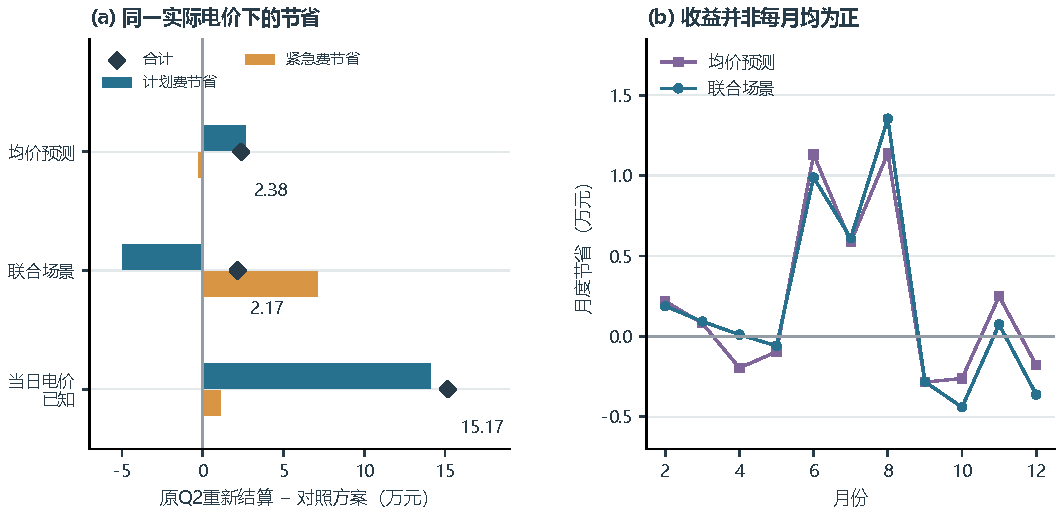
\includegraphics[width=\linewidth]{figures/07_q42_price_information.pdf}\end{center}
{\small\textbf{图注：}相对原第二问策略按附件4电价重新结算的费用节省。左图将节省分为计划费与紧急费，菱形表示合计，负值表示该项费用增加；右图展示均价预测与联合场景的月度净节省。当日电价已知为信息对照。\par}
\medskip
{\small\textbf{正文描述：}联合场景主方案的总费用为15,163,043.89元。相对原Q2重新结算，其计划费增加49,557.74元，而紧急费减少71,218.08元，净节省21,660.34元。均价预测方案在本年度比联合场景低2,122.44元，因此不能宣称联合场景取得了回测最低费用。已知当日电价对照比联合场景低130,000.71元，体现更充分价格信息的回测价值，但不构成理论最优下界。月度节省存在正负变化，年度改善不保证各月均改善。\par}
\newpage
\section*{图8　4-2：价格偏差与日前购电的时段重排}
\begin{center}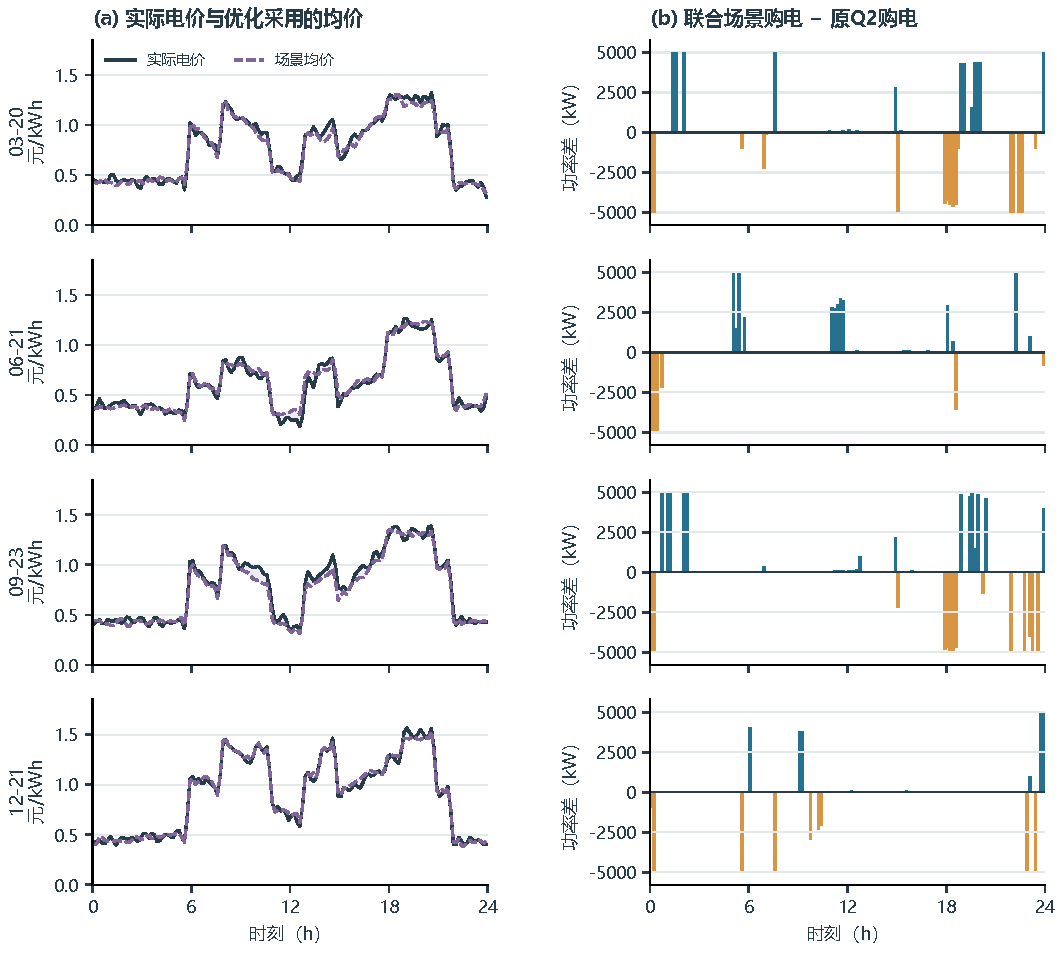
\includegraphics[width=\linewidth]{figures/08_q42_schedule_shift.pdf}\end{center}
{\small\textbf{图注：}四个指定日的实际电价、优化采用的场景均价及购电计划差异。左列阴影仅表示两条价格曲线的差距；右列为联合场景计划购电功率减去原Q2计划购电功率，蓝色为增购、橙色为少购。\par}
\medskip
{\small\textbf{正文描述：}将原第二问策略作为参照，可以观察到价格信息模型引入后购电时段发生重排。场景均价与实际电价并不处处一致，价格曲线形状接近也不保证决策完全相同。联合场景的决策还依赖价格与净负载误差的配对、储能约束及前期形成的状态，因此左、右两列用于对照现象，不将每个购电差值单独归因于同一时段的价格预测误差。此处展示的是日前计划，不应描述为当天观察实际价格后的日内修正。\par}
\newpage
\section*{图9　4-3：相对第三问的费用差额与更新收益}
\begin{center}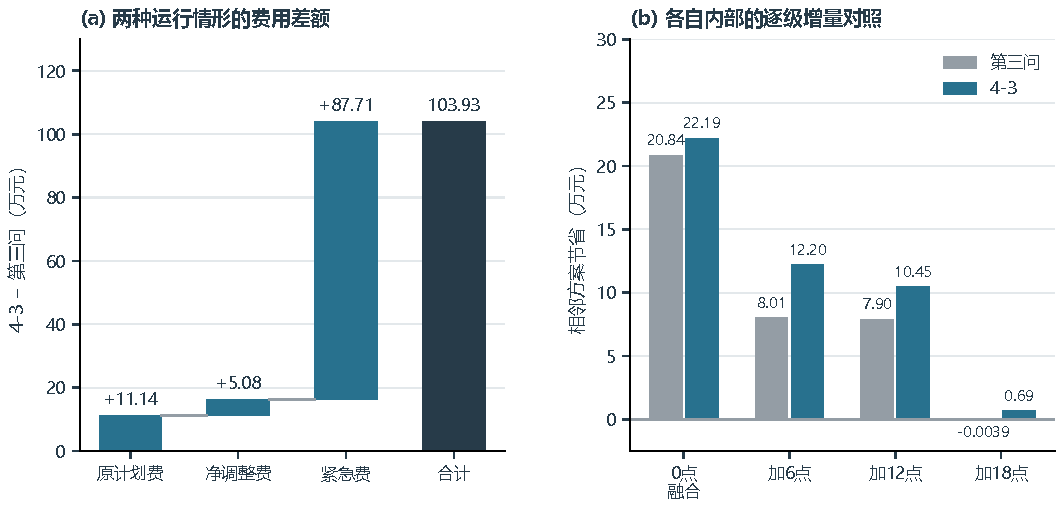
\includegraphics[width=\linewidth]{figures/09_q43_incremental_comparison.pdf}\end{center}
{\small\textbf{图注：}4-3与第三问主方案的费用差额及更新收益比较。左图按原计划费、净调整费和紧急费分解4-3减第三问的总费用差；右图分别在两问内部计算相邻更新方案之间的费用节省。\par}
\medskip
{\small\textbf{正文描述：}4-3主方案费用为15,061,735.43元，比第三问高1,039,338.45元。其中紧急费差额为877,139.21元，占总差额的84.39\%。该结果是不同电价输入及对应滚动策略共同形成的账面差异，不能全部解释为电价波动或预测误差的因果成本。在各自内部的逐级对照中，增加6点更新的节省由第三问的8.01万元变为4-3的12.20万元，增加12点由7.90万元变为10.45万元；4-3增加18点节省6,875.04元，而第三问费用增加38.88元。这表明新增调整机会的回测价值随运行情形而变化。\par}
\newpage
\section*{图10　4-3：电价、执行购电和储能状态的差异分布}
\begin{center}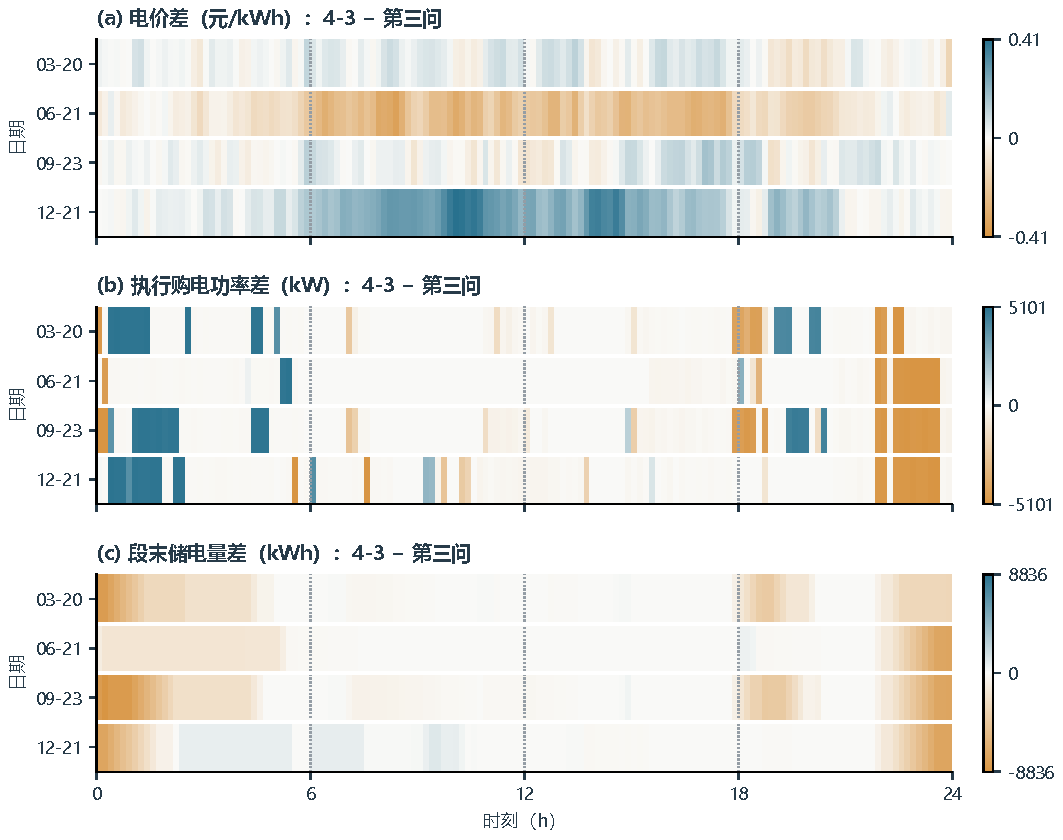
\includegraphics[width=\linewidth]{figures/10_q43_schedule_differences.pdf}\end{center}
{\small\textbf{图注：}四个指定日中，4-3相对第三问的电价、最终执行购电功率及段末储电量差值。蓝色表示4-3更高，橙色表示更低，白色表示接近零；各面板使用独立的对称色标，数值未裁剪，竖虚线为6、12、18点。\par}
\medskip
{\small\textbf{正文描述：}配对差值图保留了两问在相同实际负载与光伏条件下的时段对应关系。电价、购电与储能状态的差异具有不同的时间分布，显示调度响应包含跨时段的能量转移。各指定日的初始储电量已由此前滚动执行决定，两问并不相同，因此状态差异既包含当日决策差异，也包含前期累积影响。图中比较用于描述两套已保存运行结果，不能将某一列的颜色直接解释为另一列的因果效应。\par}
\newpage\end{document}